\documentclass[letterpaper]{article}
\usepackage{graphicx}
\usepackage{fullpage}
\usepackage{float}
\usepackage{graphics}
\usepackage{color}
\usepackage[english]{babel}
\usepackage{appendix}
\usepackage{tabularx}
\usepackage{wrapfig}


\newcommand{\HRule}{\rule{5cm}{0.1mm}}
\begin{document}
\begin{center}


% Upper part of the page
%
\includegraphics[\textwidth]{SSDDTemplateA2-img1}\\[1cm]    

\textsc{\Large University of Idaho}\\[0.2cm]

\textsc{\Large CS481: Senior Design}\\[2cm]


% Title
%{ \LARGE \bfseries Idaho Department of Health and Welfare}\\[0.4cm]
%{ \huge \bfseries Time, Accounting, and Reporting System}\\[1.0cm]
{ 
\includegraphics[scale=0.45]{logo_huge_inverse.png} }\\[2.0cm]
{ \normalsize \emph{ prepared for}}\\[0.5cm]
{ \normalsize Don Moreaux}\\
{ \normalsize Marj Sanderson}\\[0.5cm]
{ \small \emph{and}}\\[0.5cm]
{ \normalsize The Idaho Department of Health and Welfare}\\[0.5cm]
\HRule \\[3cm]

% Authors and supervisors
\begin{minipage}{0.4\textwidth}
\begin{flushleft} \large
\emph{Authors:}\\
Scott Beddall\\
Brett Hitchcock\\
Chaylo Laurino\\
Alex Nilson
\end{flushleft}
\end{minipage}
\begin{minipage}{0.4\textwidth}
\begin{flushright} \large
\emph{Advisors:} \\
Greg Donohoe\\
\bigskip
\bigskip
\bigskip
\bigskip
\end{flushright}
\end{minipage}

% Bottom of the page
{\large \today}

\end{center}
\pagebreak
\tableofcontents

\pagebreak
\section{\bfseries{Introduction}}
\subsection{\bfseries{Identification}}
This Software Design Document pertains to the Idaho Department of Health and Welfare Time, Accounting, and Reporting System. Project development for Fall Semester, 2011 is executed by Scott Beddall, Brett Hitchcock, Chaylo Laurino, and Alex Nilson. The advisor for the project from the University of Idaho is Gregory Donohoe. The project sponsor and primary client from the Idaho Department of Health and Welfare is Don Moreaux. 
\subsection{\bfseries{Document Purpose, Scope, and Intended Audience}}
\subsubsection{Document Purpose}
This document's sole purpose is to outline the scope of Idaho TARS. This outline includes, but is not limited to:
\begin{itemize}
\item Development Decisions and Rationale.
\item Architectural Specifications.
\item Detailed Design Information.
\item Locations of Other Project Resources.
\item Complete Details Regarding Project Deliverables
\end{itemize}
\subsubsection{Intended Audience for Document}
Though the TARS is to be fully prototyped by the end of 2011, it will not be completed. With that being the case, this document is aimed at any future developers or users of Idaho TARS. 

\subsection{\bfseries{Software Purpose, Scope, and Intended Users}}
\subsubsection{Software Purpose}
Idaho TARS is intended to provide time and resource tracking for contractor/non-contractor work efforts within the Idaho Department of Welfare. Work efforts must be added to time-bounded project PCA codes and approved by users with sufficient privileges. Project summaries, cost totals, user logs, and other information will then be available within TARS to authorized users. These users will be authenticated by an Active Directory interface.     

\subsubsection{Software Scope/Context}
The Idaho Department of Health and Welfare is currently utilizing a resource called Mariner for time management and accounting. The IDHW's needs, however, are significantly less than the capabilities that Mariner provides. Portfolio and Resource Management, Planning, and other features of Mariner are being paid for, but left unused. The under-utilization of Mariner, coupled with fact that the IDHW would prefer an open-source solution that meets their specific needs and workflow, motivated Don Moreaux to bring the TARS project to the University of Idaho. 

\subsubsection{Intended Users for the Software}
Intended Users of Idaho TARS are the staff and employees of the Idaho Department of Health and Welfare as well as its contractors.

\subsection{\bfseries{Definitions, Acronyms, and Abbreviations}}
\begin{center}
\begin{tabular}{| l | p{10cm} |}
\hline
MVC & Model View Controller. A design pattern used for content focused websites. Provides security through modularity, ease of maintenence, and a clear architecture.\\ \hline
TARS & Time, Accounting, and Reporting System. \\ \hline
PCA Code & Position Classification Allocation Code. \\ \hline
SQL & Structured Query Language. Used for input and retrieval of data from a SQL database.\\ \hline
IDHW & Idaho Deparment of Health and Welfare \\ \hline
Work Effort & A project. Has one or more assigned PCA Codes and a list of associated work tasks.\\ \hline
Connection String & A formatted line of text that contains all relevant connection information for a remote resource. (server, dsa) \\ \hline
LDAP & Lightweight Directory Access Protocol. A protocol used for interface with distributed directory services. (Active Directory, Apache Directory Server) \\ \hline  
DSA & Directory Service Agent. A server that specifically listens for queries via LDAP. \\ \hline
Active Directory & Microsoft Directory Services \\ \hline
Apache Directory Services & Open source LDAP alternative to Active Directory. Highly stripped down. \\ \hline
Task & An individual part of a Work-Effort \\ \hline
I-Time & Idaho Time - The system by which hours are actually submitted to the Idaho Government \\ \hline
Earnings Codes & Code describing a unit of work. VAC = Vacation. Etc.\\ \hline
IIS & Internet Information Services - Microsoft Server Infrastructure \\ \hline
.NET & Proprietary Microsoft Framework. \\ \hline
\end{tabular}
\end{center}

\subsection{\bfseries{Document Overview}}
Section 2 describes software constraints imposed by the operation environment, system requirements, and user characteristics. After this it will identify the system stakeholders and list/describe their concerns.  \\
\\
Section 3 of this document describes the system and software
architecture from several viewpoints, including, but not limited to,
the developer{\textquoteright}s view and the user{\textquoteright}s
view.\\
\\
Section 4 provides detailed design descriptions for every component
defined in the architectural view(s). \\
\\
Section 5 provides traceability information connecting the original specifications
(referenced above) to the architectural components and design entities identified in this document.\\
\\
Section 6 is a complete overview of project deliverables as well as providing an overview of the Visual Studio Solution that makes up the TARS prototype.
\\
Sections 7 and beyond are appendices including original information and communications used to create this document.

\section{\bfseries{Software Requirements, Constraints, and User Characteristics}}
The following is a compiled list of TARS requirements. Below each individual requirement is a short comment as well as a status of that requirement as of 12/7/2011.
% Generated by GrindEQ Word-to-LaTeX 2010 
% ========== UNREGISTERED! ========== Please register! ==========
% LaTeX/AMS-LaTeX

%%% remove comment delimiter ('%') and select language if required
%\selectlanguage{spanish} 

\noindent \textbf{Current Idaho TARS Requirements}\\
\\

\noindent \textbf{PCA-1}

\noindent Users with the proper permissions must be able to manually enter PCA codes in a form that meets DHW standards.\\

\noindent Status: \textbf{In Progress.  All of the core functionality exists to add, edit, and delete PCA codes to and from the database.  However, there is no user friendly interface.}\\
\\
\noindent \textbf{PCA-2}

\noindent Users with proper permissions must be able to manually tie work effort(s) to valid PCA.

\noindent \textit{This provides the ability to correctly connect the PCA code(s) to work, and ensures we are correctly accounting for what costs are allocated to what work. Work can be project related, a maintenance activity, or a non-productive activity such as meeting time.}

\noindent Status: \textbf{In Progress.  All of the core functionality exists to create associations between PCA codes and Work Efforts.  However, there is no user friendly interface.}\\

\noindent \textbf{PCA-3}

\noindent The system must provide a mechanism for time bounding PCA codes - with the ability to "deactivate" a code prematurely and an open "end" date.

\noindent \textit{Codes need to have start and end dates assigned to them, and depending upon user permissions, those dates may or may not be editable. Do not mimic MS Projects start and end date functionality.}
\noindent Status: \textbf{In Progress.  There exists a flag to indicate that a PCA code is active or not.  However, there exists no user interface to manually deactivate PCA codes nor is there any automated system to check PCA code's time bounds.}\\


\noindent \textbf{PCA-5}

\noindent The system must provide a mechanism for preventing time to be allocated to expired PCA codes.

\textit{No Comments}

\noindent Status: \textbf{In Progress.  The flag exists but as of yet no check is made because no permanent user interface yet exists.}\\
\\
\noindent \textbf{PCA-6}

\noindent The system must allow multiple PCA to be assigned to a work effort, over the life of the effort/project.

\textit{No Comments}

\noindent Status: \textbf{In Progress.  The functionality exists to allow multiple associations as well as the removal of associations but there is no visual interface for it yet.}\\

\noindent \textbf{PCA-7}

\noindent Must be able to assign one or more PCA codes to work effort (split \% allocation across multiple PCAs which can change during life of work effort).

\noindent \textit{In the case where a work effort is tied to more than one PCA, there needs to be some mechanism for determining how the work is partitioned between the two.}

\noindent Status: \textbf{In Progress.  Some functionality exists but is not complete and no visual interface exists.}\\

\noindent \textbf{PCA-8}

\noindent Must allow work to be assigned to other entities outside DHW.

\noindent \textit{Provides a means of identifying between DHW and non-DHW contractor hours.}

\noindent Status: \textbf{In Progress.   Work efforts can be associated to a user but there currently exists no visual way to manually associate work to someone other than the user currently logged in.}\\



\noindent \textbf{PCA-9}

\noindent Must allow work to be associated with multiple divisions or the enterprise.

\textit{No Comments}

 Status: \textbf{Incomplete.}\\
\\
\noindent \textbf{DATA-1}

\noindent The system shall track date specific vendor and employee/contractor information.

\noindent \textit{Provide some mechanism for tracking employment status and changes. For example, when a contractor is hired on as state staff, or changes vendors, TARS would allow that information to be entered and tracked. Need data elements.}

\noindent Status: \textbf{In Progress?  Employee Data is stored in the Active Directory.  If something separate is needed than it will need to be added as there is currently no functionality for the storage of data not associated to PCA Codes, Work Efforts, or Tasks.}\textit{}

\noindent \textit{}

\noindent \textbf{DATA-2}

\noindent The system shall allow for some description of work or project to be entered and attached.

\textit{Provide ability to describe the work effort in general terms.}

Status: \textbf{Complete.  There exists a field for comments to be added to hours logged.}\textit{}\\

\noindent 

\noindent \textbf{DATA-3}

\noindent The system shall be consistent with I-Time data.

\noindent \textit{Use the codes and logic from I-Time (see DAT-7 and REP-2) codes are Earning Codes - 3 digit}

\noindent Status: \textbf{Tabled.  This aspect of the project was declared to be outside of the scope of this semester and was tabled.}\textit{}\\

\noindent 

\noindent \textbf{DATA-4}

\noindent The system shall provide a means to replicate last week's assignments (repeating tasks can auto fill)

\noindent \textit{For those staff/contractors that repeat most work efforts each week, having the ability to replicate the proceeding week saves data entry time.}

\noindent Status: \textbf{In Progress.  Some functionality exists but a controller will need to be added to pull the last approved entry from the database upon request by the user.  Also a view will be needed.}\textit{}\\

\noindent 

\noindent \textbf{DATA-5}

\noindent The system must have a method that allows staff to create work effort, and self-assign.

\noindent \textit{Users would have the ability to create work effort, then assign themselves to that effort. Clarification - Staff can self assign to a particular work effort, Mgrs and Admin only can CREATE a work effort with a PCA}

Status: \textbf{Complete.}\textit{}\\

\noindent 

\noindent \textbf{DATA-6}

\noindent Must be able to track work effort for resources, depending upon their assignment, that are either cost allocated or not cost allocated. 

\noindent \textit{Clarification - Cost allocated codes are PCA codes (all work is entered unto I-time as ACT, all non-work time captures is by Earnings Codes.}

Status: \textbf{In Progress.  The functionality exists but there are no visual elements yet.}\textit{}\\

\noindent 

\noindent \textbf{DATA-7}

\noindent Must be able to break time out by time codes for non-work efforts, such as Vacation, Sick, LWOP, (match I-Time data since this is the system of record)

\noindent \textit{Need to understand data requirement for I-Time if the plan is to eventually interface with I-Time.} \textit{All time in I-time is seen as worked or non-worked.  All "work" is coded to ACT, non work is coded to various codes.}

\textit{ }Status: \textbf{In Progress.  The functionality exists but there are no visual elements yet.}\\

\noindent 

\noindent \textbf{DATA-8}

\noindent Users shall have the ability to close tasks and activities on their timesheet, and reopen if needed.

\noindent \textit{This is separate from the open/closed PCA codes.  A user may no longer be working on a particular project or investment so they want to close it out on their time sheet.}

\noindent Status: \textbf{Progress.  This level of visual design was beyond the scope of this semester.  However, some functionality exists.}\\

\noindent 

\noindent \textbf{DATA-9}

\noindent The system shall provide some mechanism (configurable dropdown) for grouping of business, program, and function of work.

\textit{Need to be able to add/edit/delete values into those lists. This is grouping for a work effort.}

\noindent Status: \textbf{Progress.  This level of visual design was beyond the scope of this semester.  However, some functionality exists.}\\

\noindent 

\noindent \textbf{DATA-10}

\noindent Audit trail data shall include the information that was updated, modified/deleted, date created, and by whom for each item determined to be auditable. The TARS team has proposed storing every SQL query executed by a user.

 \textit{Need to define what will be included in the audit trail.}

\noindent Status: \textbf{Complete.  The History table exists and is populated as the system is used but no visual interface exists to view said histories.}\textit{}\\

\noindent 

\noindent \textbf{DATA-11}

\noindent Data for staff and projects shall include the ability to store links and attachments

\noindent \textit{Related in part to DAT-2, in that it provides a means for capturing work and project information that describes the work effort.}

\noindent Status: \textbf{In Progress.  Some functionality exists but nothing has been done yet concerning storing files} \\

\noindent 

\noindent \textbf{DATA-12}

\noindent The system must allow for future time entry

\noindent \textit{Any user should be allowed to enter time against a work effort, in advance of the current week.}

Status: \textbf{Complete.  No restriction is made on how far ahead time can be entered for.  Some  might be warranted.}\\

\noindent 

\noindent \textbf{DATA-13}

\noindent Must prevent work efforts to exist in the system unless they are tied to a PCA code.

\noindent \textit{ PCA codes and work efforts (tasks, \dots ) are all time bounded in this system. To prevent inaccurate recording of time allocated to an effort, some automated process of preventing expired or deactivated objects should be developed. System must also allow non-work time to be recorded using Earnings Codes (I-Time) such as VAC, HOL, etc.}

\noindent Status: \textbf{In Progress.  The functionality to make associations exists but not to require them.}\\

\noindent 

\noindent \textbf{REP-1}

\noindent All data for reporting shall be extracted via external source (EDW. Excel, etc.).

\noindent \textit{Team sees no need to build in reporting in TARS, since we can generate reports with Business Objects, or other database connections. }

\noindent Status: \textbf{Inactive.   This was declared out of the scope of this semester and has not been considered at all yet.}\\

\noindent 

\noindent \textbf{REP-2}

\noindent Must allow users to create a view of their I-Time timesheet.

\noindent \textit{I-time is a separate timesheet, into which users also enter time for payroll accounting. (This requirement will be prioritized at the very bottom.  Isn't needed until we interface with I-Time)}

\noindent Status: \textbf{Inactive.   This was declared out of the scope of this semester and has not been considered at all yet.}\\

  

\noindent \textbf{REP-3}

\noindent Reports must be real-time, reliable, and accurate. Includes exports to csv, Excel.

\noindent Speaks to having a simplified database schema, one that allows external connections (ODBC, etc.) to easily connect and extract data for reporting purposes. Reports will be created using Business Objects, not in TARS

\noindent Status: \textbf{Inactive.   This was declared out of the scope of this semester and has not been considered at all yet.}\\

\noindent 

\noindent \textbf{REP-4}

\noindent The system must prevent time entry to a user's time sheet once the week period has cycled through. (a week is a calendar week, and cycled through means that the time sheet has been approved by management)  Admin role should have the ability to "unlock" the time period and allow time sheet changes.
	
\noindent(Note: This is not to be confused with the open/close time periods of PCA codes)

\noindent Status: \textbf{In Progress}\\

\noindent

\noindent \textbf{VIEW-1}

\noindent Must have a sort and group function that allows work effort to be grouped by application, division, manager, etc.

 \textit{No Comments}

\noindent Status: \textbf{In Progress.  The only views currently are for testing purposes.  Thus all the ``View'' requirements are In Progress.  Visual Design will be a primary focus of the second semester.}\textit{ }\\

\noindent \textit{}

\noindent \textbf{VIEW-2}

\noindent The system must allow a user the ability to create a custom view of the data.

\noindent \textit{Users should be able to slice data, such as work effort by staff member over a date range. Users should only be able to see and customize their own data unless they are mgrs or admin and the view should persist.}

Status: \textbf{See View-1}\\

\noindent 

\noindent \textbf{VIEW-3}

\noindent Must allow users to easily size windows

 \textit{No Comments}

\textit{ }Status: \textbf{See View-1}\textit{}\\

\noindent 

\noindent \textbf{VIEW-4}

\noindent Must be able to limit view of information presented to user to what is pertinant to that user's role.

\textit{This requirement is tied to VIEW-2 in that it limits the range of customization of a view.}

Status: \textbf{See View-1}\\

\noindent 

\noindent \textbf{VIEW-5}

\noindent The system shall provide search/find functionality to locate work efforts, with minimal amount of navigation (task actions$<$=4 clicks/pages/dialogs)

\noindent \textit{The number of clicks should be proportional to the frequency of the TARS tasks. In other words, TARS tasks that users frequently execute, should have the fewest navigation steps. Users can only create a view of their own data. Mgrs should be able to group their staff for time approval.}

\noindent Status: \textbf{See View-1}\\

\noindent 

\noindent \textbf{SEC-1}

\noindent Must authenticate using LDAP.

\noindent \textit{Initially authenticating to Active Directory was a requirement. For now, we are using Apache DS to authenticate users. }

\noindent Status: \textbf{In Progress.  Currently authenticates using LDAP.  Will need to be modified to authenticate to Active Directory.}\textit{}\\

\noindent \textit{}

\noindent \textbf{SEC-2}

\noindent Must have a role-based permissions security.

\noindent \textit{Would like to have the ability to create new roles, and assign permissions to that role. For example, an Administrator have rights to edit/delete PCA codes and users, while an Individual Contributor would not have those rights. Basic role set would include Administrator, Manager /Approver, and Worker.}

\noindent Status: \textbf{Inactive.  This is taken care of by the Active Directory system and thus has been striken from this list.}\\

\noindent 

\noindent \textbf{SEC-3}

\noindent The system shall allow for automated closure of time periods for PCA and work efforts, with administrator ability to manually reopen \& close for edit \& approval

\noindent \textit{Tied to DAT-13 in preventing work efforts and codes from lingering when they are no longer active. This is also an example of a permission element in the role-based security profile.}

\noindent Status: \textbf{In Progress.  The flag to mark a PCA code and Work Effort as closed and the field to set the time bounds exist.  However, no automated system to set that flag when the time runs out has been implemented.}\\

\noindent 

\noindent \textbf{NAV-1}

\noindent The system must allow each user the ability to navigate easily by logic/functional areas, ie. Staff demographics, projects, work items/areas, time entry, etc.

 \textit{No Comments}

Status: \textbf{See View-1}\textit{}\\

\noindent 

\noindent \textbf{NAV-2}

\noindent Must automatically display current week when entering timesheet data.

 \textit{No Comments }

\textit{ }Status: \textbf{See View-1}\textit{}\\

\noindent 

\noindent \textbf{WKF-1}

\noindent Must have notifications (via email, context, \dots ) triggered by certain events such as timesheet submittal, approvals, PCA expiration, etc.

\noindent \textit{The current system auto-sends emails to notify users of their due timesheets, though the message is not tied to timesheet status (i.e. you get the mail even if your timesheet was submitted for that week). One notification would be to the worker who has NOT submittee his/her time by end of day on Saturday.}

\noindent Status: \textbf{Inactive.  This was declared out of the scope of this semester and was not addressed.}\\

\noindent 

\noindent \textbf{WKF-2}

\noindent Users with permissions, must have the ability to approve TARS weekly submittals

\noindent \textit{Assumes ability to view other's timesheets based on your role permission. Rejected timesheets will provide notification to the submitter.}

\noindent Status: \textbf{In Progress.  The field to flag a timesheet as approved exists but there is no visual way to set that flag.}

\section{Software Architecture}
\subsection{Server Architecture - Microsoft Internet Information Services 7} 
One of the IDHW's requirements for the this project is the use of Windows Server infrastructure. In this case the TARS development team will use Microsoft IIS7. Microsoft's Internet Information Services server is a modular, intuitive server application. New considerations must now be applied, however. IIS7, being a Microsoft product, uses Microsoft development software. Namely:
\begin{itemize}
\item C\# 
\item ASP.NET
\item Visual Basic/VB.NET
\item .NET Development Framework
\item Active Directory Services
\end{itemize} 
TARS will be developed using all these technologies, as well as the IIS7 Model-View-Controller application. The MVC application will be described in detail in the next section. 

\subsection{Model-View-Controller}
Most of the heavy-lifting for TARS will be present in the display and interaction with large amounts of data. This problem is what the Model-View-Controller design pattern was created for. The idea is that each word in the acronym: Model, View, and Controller each represent a component that handles a different aspect of the display process.\\
\\

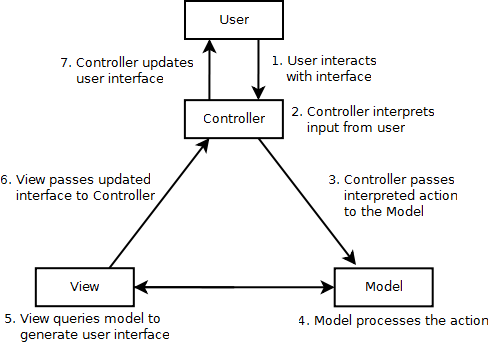
\includegraphics[scale=0.6]{../design/images/mvc.png}\\
\\
Advantage of Model-View-Controller architecture:
\begin{itemize}
\item Separates the user interface from the logic used in the database.
\item Allows for independant development, testing, and maintenance of these seperate parts of the application.
\end{itemize}
\subsubsection{Controller}
A Controller receives input from the user and converts it to instructions for the Model and View components. Most MVC's use the first argument after the website URL as the controller call. In our case:\\
\begin{verbatim}
http://idahotars.com/home
\end{verbatim}
Will load the ``home'' controller default function (Index). The second entry in the url after the controller selection will select the specific function in the controller. Any subsequent entries will then make up arguments to the specific function.\\
Load the viewTimeSheet function in the user controller:
\begin{verbatim}
   idahotars.com/user/viewTimeSheet 
\end{verbatim}
Load the viewTimeSheet function in the user controller with arguments 10 and 20:
\begin{verbatim}
   idahotars.com/user/viewTimeSheet/10/20
\end{verbatim}
This configuration can be viewed or modified in ``global.aspx.''  

\subsubsection{Model}
The Model manages database queries and assembles data for use elsewhere in the MVC. However, in the MVC3.0 extension specific to IIS7, there is a slight oddity when it comes to the Model component. That is, the Model doesn't actually execute any of the database interaction. Instead, the Models are used specifically as database table schemas, giving TARS a way to know what the remote tables look like. The actual interaction is carried out by Database Contexts. (DbContext class)
\subsubsection{View}
Views render the data received from the Models into viewable web pages.
\subsection{SQL2008 Database}
Though IIS can utilize any format of SQL Database, the IDHW requires that TARS use SQL2008. Any queries made by the MVC will be carried out by the "Model" component of the MVC. \\
\\
\subsection{Active Directory}
The IDHW uses Microsoft Active Directory for their user authentification. With that infrastructure already in place, it is logical to use the same for Idaho TARS. To authenticate users of TARS, there will be three new Active Directory groups added: TARSAdmin, TARSManager, and TARSUser. If a given user is part of any of these three groups, they will be allowed access to TARS based upon their group. \\
\\
To provide this functionality, the TARS development team wrote a helper class that can be used when an Active Directory connection is needed. This ``LDAPConnection'' class can be invoked within any controller, so long as ``TARS.Helpers.LDAPConnection'' is referenced.\\
\\
Primary functions for now are:
\begin{verbatim}
LDAPConnection() //constructor, initiates variables needed for a connection
boolean requestUser(string user, string password); //returns true if the user/password combo exists
string requestRole(string user); //returns which group a user is part of
\end{verbatim}
All these functions create an LDAP connection, query the DSA, and close the connection. The user of this helper class need not ever understand what is going on under the hood to use it correctly. 

\subsection{Security}
While Idaho TARS will be used internally, there is still a security risk. The system may not be dealing with any highly confidential info, but TARS will have access to government resources like the IDHW Active Directory and I-Time interfaces.\\
\\
To prevent easy exploitation of the TARS databases, all queries to the database will be centralized in Model. This will will not only make the team's code simpler, but also make it more secure. Centralized queries allow us to easily adopt a strong security stance. In addition, TARS uses DbContexts for database interaction. With that being the case, no SQL is ever directly executed from TARS. This significantly reduces the risk of SQL Injection attacks.


\subsection{Browser Interface}
Though it is probably already indicated by the server architecture, the development team must make it clear that this software is being developed for a web interface. This will eliminate many of the dependencies that are inherent to a system launched from a binary. The development team is developing this project to meet the following end system requirements:
\begin{itemize}
\item 1024x768 monitor resolution
\item Google Chrome
\item Mozilla Firefox
\item Internet Explorer 7 and up
\item Safari
\item Compliant with W3C standards
\end{itemize}
\section{Design Descriptions}
\subsection{Model-View-Controller Modules}
\subsubsection{Global Scripts and Config Files}
There are two extremely important configuration files within the Visual Studio solution. Unfortunately, two both named ``Web.Config.''\\
\\
The first Web.Config is present in projectBase/Views/Web.Config. This config file handles various view configurations that affect TARS visually.\\
\\
The second Web.Config is present in projectBase/Web.Config. It handles project level configuration; most importantly including the extremely important database connection strings. \\
\\
The third, and by far the most important config file is projectBase/Global.aspx.
This contains the functions that control routing for the entire MVC. This job includes determining routing to controllers, filtering requests, and registering the initial routes on a default request for idahotars.com.

\subsubsection{Controllers}
These controllers do not yet have a finalized set of associated functions and variables. When these are complete a full description will reside here.
\begin{itemize}
\item HomeController
\item UserController
\item ManagerController
\item AdminController
\item AccountController
\end{itemize}
The home controller is the default page in the case that a user is not logged in. It also provides the entry point to TARS when a controller is not specified. \\
\\
AccountController provides login functionality. This includes calling the LDAPConnection helper class to authenticate users. AccountController was provided by a base example of an MVC, but is modified to serve the TARS specific needs.\\
\\
UserController inherits from the default MVC Controller class as well as providing basic functionality for a normal user.\\
\\
ManagerController inherits from UserController, but adds a couple more abilities that managers need as per the requirements specification.\\
\\
AdminController inherits from ManagerController, inheriting all functionality as well as providing any and all administrative functions that are needed by TARS admin. Having these inherited privileges ensures that forced permission traversals will be almost impossible.\\ 
\begin{verbatim}
Home Controller //Default controller called when visited TARS 
                //for the first time or when not logged in.

User Controller
 -> ManagerController
  -> AdminController

\end{verbatim}
\subsubsection{Models}
\begin{itemize}
\item AccountModels (provided by IIS7 MVC)
\item History
\item Hours
\item PcaCode
\item PCAWE
\item WorkEffort
\item TARSUser
\end{itemize}
These items do not inherit from the default Model class. In addition, each class has an associated DbContext class in the same file. Example:
\begin{verbatim}
public class PCA_CodeDBContext : DbContext
{
   public DbSet<PcaCode> PCA_CodeList { get; set; }
}
\end{verbatim}
These connections are not conventional classes or objects. To indicate this, their naming conventions are slightly more verbose. A DbContext creates a new context instance that utilizes an existing Database Connection String (located inside web.config) to create a connection to a SQL Database.
\subsubsection{Views}
\begin{itemize}
\item Every controller has an associated View. Located in their respective folders. Manager example:
\begin{verbatim}
Views/Manager/___.cshtml 
   ///where ___ is a view associated with a given function within the controller
\end{verbatim}
\end{itemize}
\subsection{SQL2008 Database Schema and Interface Description}
As mentioned above in the Software Architecture section, TARS will use a SQL2008 database to store all interactions other than User Info (handled by Active Directory). Before outlining the Database Schema, it would be wise to fully describe the thought process of the development team.\\
\\
Stripped down to its most base parts, TARS is simply a database interface through which users can log and retrieve hours to and from work efforts. These ``Work Efforts'' are simply general projects that can have hours of contractor/non-contractor work added to their totals. For instance, there might be a Work Effort that is assigned its own unique ID and whos description is ``Document the latest changes to the TARS SDD.'' Any employees who wish to log their hours will find the Work Effort's ID, add their hours along with other relevant data, and submit their entire timesheet for approval. \\
\\
The Work Effort to ``Document the latest changes to the TARS SDD.'' now has hours logged on it and waiting for approval. A user with the correct Active Directory permissions (part of group TARSManager or TARSAdmin) can now go check the status of the Work Effort, and approve any pending hours waiting on it. The development team has chosen to add all hours, approved or not, to the Work Effort's database table. A simple boolean present as a column in the table will ensure that filtering by approved/un-approved will be a simple task.\\
\\
Unfortunately, the process is not done. Now that a Work Effort has hours charged to it, how can the accounting department charge these expenses? The simple answer is, they can't yet. To provide that functionality, PCA Codes must be assigned. This introduces another database table, as one PCA Code may have multiple Work Effort associations; just as one Work Effort may be associated with multiple PCA Codes.\\
\\
One final note about the Work Efforts and PCA Codes is needed. The requirements state that they both must be time-bounded, capable of early expiration, and renewable. \\
\\
In addition, for each of these Models, there is also a modification to their paramaterized DbContexts. That is, DB.saveChanges() is overwritten to save a new entry in the History table before calling super.saveChanges(). \\
\\
Addendum for 11/1/2011. The stakeholders introduced the concept of ``tasks.'' There will be a default set of tasks for every work effort, but members of the ``administrator'' Active Directory group will have the ability to add or remove these ``tasks'' from a given work effort. While the development team at one point believed it possible to create Tasks functionality without another database table, the belief was quickly proven infeasible. With that being the case, a new table was added.\\
\\
Addendum as of 11/23/2011. The TARS development team has learned that while the Active Directory DSA will service user/password requests, TARS will be unable to push any changes to the Directory. With that being the case, the development team quickly deduced that yet another database table would be needed. Namely, the ``TARSUser'' table. This table will store unique userids as well as any web and role configuration information that may be needed by TARS in the future. For now, the development team is simply using it to store Role information. Later on, the configuration storage will be utilized by the next team.

\subsubsection{TARS Database Schema}
%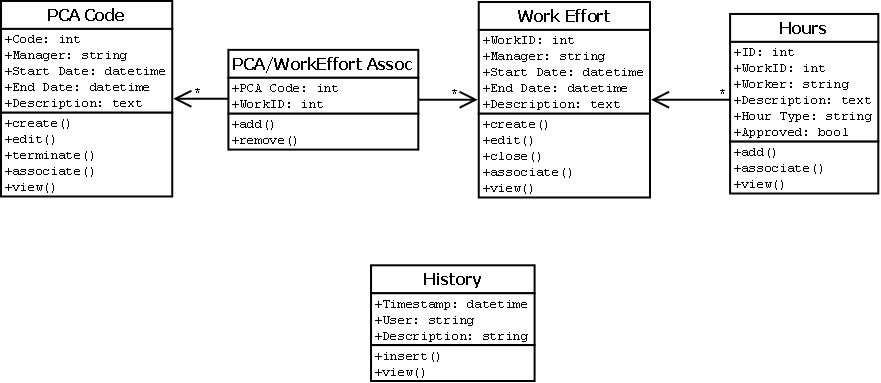
\includegraphics[scale=0.4]{../design/images/class_diagram_1.png}
\begin{centering}
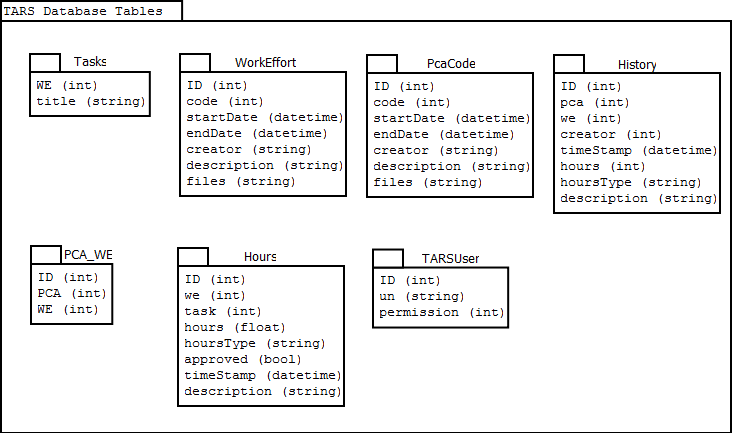
\includegraphics[scale=0.64]{schema.png}
\end{centering}
\subsection{Naming Conventions}
All defined classes and objects will use capitalized camelcase, with their first letter a capital as well.\\
\\
Local Variables and instances of classes will use camelcase also, neglecting the capitalization of their first letter.
\begin{verbatim}
class Manager : Controller
{
    public int id;
    public bool approved = FALSE;
    public string hoursType;
}
\end{verbatim}

\section{Tracability Information}
All effort on the project may be tracked via the project GitHub repository: github.com/ICBM/TARS\\
\\
The project website resides at: http://seniordesign.engr.uidaho.edu/2011-2012/CostManagement/\\
\\ 
Client requirements changes will be handled via email. Current progress on requirements as well as the requirements changelog is available at: github.com/ICBM/TARS/blob/master/doc/requirements\_summary.docx\\

\section{Deliverables}

\subsection{Deliverables Overview}
At the end of the first semester the TARS team turned over the following deliverables to be passed on to the next semester's team for completion; This Design Document, Client Requirement Documents, Meeting Minutes, Tutorials, Prototype Source Files, Requirements Summary, and our GitHub Repository. For exact locations, check the ``GitHub Locations of Importantance Section''\\
\\
This Design Document contains all of the conceptual and technical designs for this project.  It also includes various Client restrictions on software and platform for the project.  For further details please read the document.\\
\\
The Client Requirement Documents outline the Client's desired functionality of the system.  It is broken down into six parts: PCA, Data, Reporting, View, Security, Navigation, and Workflow.  This document was provided to us by the Client.  It has been updated several times as requirements have been added or altered.\\
\\
All of the Minutes of our meetings with our clients as also been added.  They show the changes in the requirements over time and contain clarifications to questions the client may have had during the course of the project.\\
\\
Extensive trial and error was involved in setting up our machines to be viable development platforms based on the restrictions laid out by the Client.  To prevent the next team from having to deal with the same problems already dealt with, the TARS development team has created several tutorials to help smooth the process.\\
\\
A functioning prototype has also been produced.  It includes all the primary models and controllers but has only rudimentary views and testing.  The source code has been provided as has a Microsoft Visual Studio solution.  The full details concerning the functional state of the prototype in relation to the full project requirements are laid out in the Requirements Summary document as well as the Requirements section of this document.\\
\\
The Requirements Summary is a combination of the Client Requirement Document and a full summary of our prototypes functionality.  It explains in detail the current status of every requirement.\\
\\
The final deliverable is the TARS GitHub Repository.  It has been the primary location for all collaborative work.  It is an open source repository as the client desired to make the source code open-source.  Maintaining private collaborators costs twelve dollars a month and will need to be transferred to the new team as soon as they take up the project.\\
\\
\pagebreak
\subsection{Prototype Deliverable Detail: Visual Studio Solution Architecture}

{
\begin{wrapfigure}{r}{0.33\textwidth}
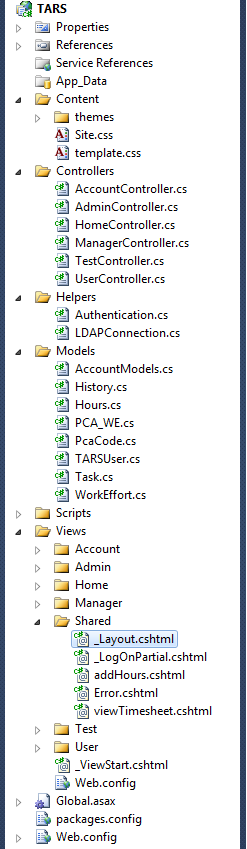
\includegraphics[scale=0.9]{project_organization.png}
\end{wrapfigure}
\paragraph{}
At the topmost level of TARS are a variety of folders as well as configuration information for the project as a whole.
\paragraph{Web.config} contains all configuration information for the webpage. The primary use of it so far has been to add Connection Strings to allow for database connection.
\paragraph{Content folder} contains the CSS data for the website.
\paragraph{Controllers folder} contains all Controllers for the project, which are described above.
\paragraph{Helpers folder} contains all helper classes under the namespace TARS.Helpers. Included thus far are the Authentication and LDAPConnection classes.
\paragraph{Models folder} contains all model classes, which are described above.
\paragraph{Views folder} contains all relevant views, which are organized into 
\\subfolders according to the Controller they belong to. The exception to
\\this is the Shared folder, where a controller will look for a view if it
\\is not found in its own specified folder. This is very useful for views 
\\that are spread unchanged between permission classes, such as 
\\viewTimesheet. As well, it should be noted that \_Layout provides the
\\default layout for ALL pages.
}
\pagebreak
\paragraph{}
So, for the server to generate a sample page to the user (let's say webroot/Manager/viewWorkEffort?id=1), it will follow this general process:
\begin{itemize}
\item Open the appropriate controller, in this case Manager. The server will only call the constructor when it is first created, not on every new page load.
\item Check the Manager controller for a public function called viewWorkEffort. If this function were not found, it would check under the User controller, since Manager inherits from User.
\item In this case, Manager has viewWorkEffort overridden from User to enable Edits, so it will load this function and check for proper arguments. 
\item The function declaration is expecting an \emph{int id}, which we have passed. So now, the function will load.
\item In the function body, the function will make an Authentication class and check to make sure the user logged in actually is a Manager or Admin. If not, it will redirect the User to an error or login page.
\item To obtain information about Work Effort \# 1, the function will create an empty WorkEffort class and fill it from WorkEffortDBContext.WorkEffortList.Find(1); Behind the scenes, WorkEffortDBContext is connecting to a server according to the connection string in Web.config, and looking for a table called dbo.WorkEfforts.
\item At this point, any other information can be passed to the View by adding it to ViewBag. EX: ViewBag.newitem = ``Hello.'';  //Runtime type checking on this.
\item The View now has all needed information from the Model and ViewBag, so output everything in the View and display to the user.
\end{itemize}
\begin{centering}
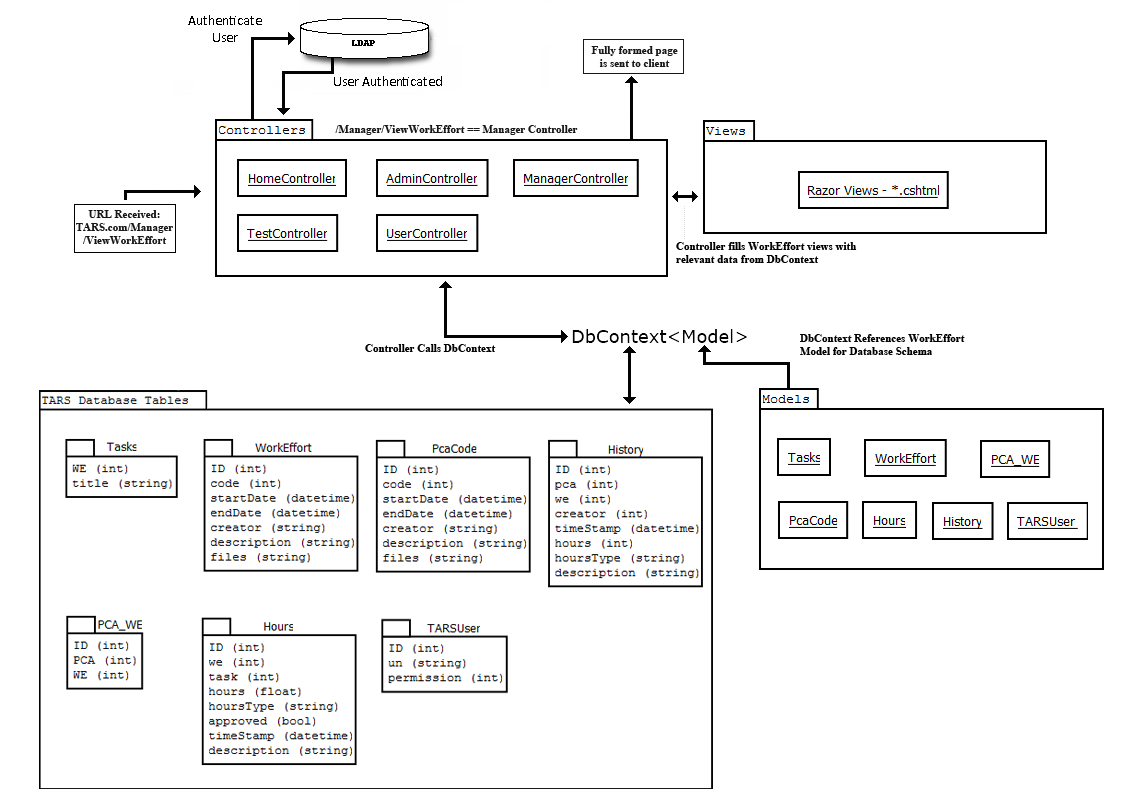
\includegraphics[scale=0.4]{erd_flow.png}
\end{centering}
\pagebreak


\subsection{GitHub Locations of Importantance}
The root directory is present at github.com/ICBM/TARS
\begin{itemize}
  \item SSD: /doc/ssd.tex -- /doc/ssd.pdf
  \item Meeting Minutes: /minutes
  \item Tutorials: /doc/Tutorials-Resources/
  \item Prototype: /TARS
  \item Requirements Summary: /doc/requirements.docx
  \item Client Requirements Document: /doc
  \item Contact Information: /contact\_info.pdf
  \item SQL Config Dumps: /doc/Tutorials-Resouces/SQL/
  \item LDAP Config Dumps: /doc/Tutorials-Resouces/LDAP/
\end{itemize}


\section{Appendix A: Use Cases} 
\paragraph{Login}
\begin{enumerate}
\item Click the "Login" button
\item Enter username and password
\item Hit Enter or click "Submit"
\item System authenticates and redirects to home page.
\end{enumerate}

\paragraph{Adding new PCA code.}
\begin{enumerate}
\item Select "Add PCA"
\item System loads PCA form
\item Fill in form, including time bounds for the PCA code
\item Press "Submit"
\item System updates tables and redirects to new PCA display page
\item A request to the financial department will be automatically dispatched. PCA codes are not actually generated by TARS.
\end{enumerate}

\paragraph{Deactivating PCA code}
\begin{enumerate}
\item Select desired PCA code
\item System loads PCA display page
\item Click deactivate
\item Confirm deactivation.
\item System updates tables and locks PCA code.
\end{enumerate}

\paragraph{Adding Work Effort}
\begin{enumerate}
\item Select "Add Work Effort"
\item System loads Work Effort form
\item Fill in form
\item Associate desired PCA code or codes, if multiple PCA codes are chosen a percentage of work effort may be set for each
\item Associate entity or entities
\item Click "Submit"
\item System updates tables and redirects
\end{enumerate}

\paragraph{Updatinging Work Effort}
\begin{enumerate}
\item Select "Update Work Effort"
\item System loads Work Effort form
\item Make Changes in form
\item Click "Submit"
\item System updates tables and redirects
\end{enumerate}

\paragraph{Adding Hours}
\begin{enumerate}
\item Select "Add Hours"
\item System loads Work Effort Selection form
\item Select Work Effort
\item System loads Hours form
\item Fill in form or select "replicate" to fill with previous weeks data
\item Click "Submit"
\item System updates tables and redirects
\end{enumerate}

\paragraph{Approving Hours}
\begin{enumerate}
\item Select "Approve Hours"
\item System loads hour approval form and fills with items needing approval
\item Select item
\item Select "Approve" or "Disapprove"
\item System updates tables and redirects back to hour approval form
\end{enumerate}

\paragraph{Adding Tasks}
\begin{enumerate}
\item Select "Add Tasks"
\item System loads Work Effort Selection form
\item Select Work Effort
\item System loads Task List form
\item Add desired tasks
\item Click "Submit"
\item System updates tables and redirects
\end{enumerate}

\paragraph{Edit/Update Employee/Contractor Data}
\begin{enumerate}
\item Select desired entity
\item System pulls data from database and loads Entity Form
\item Edit/Update as desired
\item Click "Update"
\item System updates table and redirects.
\end{enumerate}

\paragraph{View History}
\begin{enumerate}
\item Select "View History"
\item System loads History Search form
\item Enter Search Criteria
\item System loads Search Result form and fill with data
\end{enumerate}

\paragraph{The system must allow for future time entry}
\begin{enumerate}
\item Select ``Add Work Effort''
\item Fill in form, making sure to add the effort to the correct date.
\item Click ``Submit''
\end{enumerate}

\paragraph{All data for reporting shall be extracted via external source (EDW. Excel, etc.).}
\begin{enumerate}
\item Under a given PCA code or work effort, select ``Get Data Report''.
\item The system will then generate a copy of the data in EDW or Excel format.
\item User saves the copy at a destination of their choosing.
\end{enumerate}

\paragraph{Must allow users to create a view of their I-Time timesheet.}
\begin{enumerate}
\item User logs in.
\item On the user's personal page, select ``Get I-Time Report''.
\item The system will then generate a copy of the data for viewing.
\end{enumerate}

\paragraph{Must have a sort and group function that allows work effort to be grouped by application, division, manager, etc.}
\begin{enumerate}
\item User logs in.
\item User selects ``My Work Efforts''
\item System generates list of all work efforts related.
\item User selects to sort by name, application, etc.
\item System sorts and redisplays work efforts in the proper order.
\end{enumerate}

\paragraph{The system must allow a user the ability to create a custom view of the data.}
\begin{enumerate}
\item User selects a PCA code or Work Effort code
\item User selects ``Get Data Report''.
\item User enters custom settings and hits ``Select''.
\item System generates report.
\end{enumerate}

\paragraph{Must allow users to easily size windows}
\begin{enumerate}
\item User resizes browser, which will resize the web interface.
\end{enumerate}

\paragraph{The system shall provide search/find functionality to locate work efforts, with minimal amount of navigation (less than 5 clicks per important action)}
\begin{enumerate}
\item User logs in.
\item User navigates to a work effort by...
\begin{itemize}
  \item Clicking on a link in the ``My Recent Work'' bar.
  \item Entering a Work Effort code or PCA code in the Search bar on the top.
    \end{itemize}
\end{enumerate}



\section{Appendix C: Reference Links}
Unit Testing ASP.NET MVC\\
\small{http://msdn.microsoft.com/en-us/magazine/dd942838.aspx}\\
\\
SQL2008 integration w/ IIS7 MVC reference\\
\small{http://blog.evonet.com.au/post/Setting-up-SQL-Server-2008-for-an-ASPNET-website-on-IIS-70.aspx}\\
\\
SQL2008 St15udio Manager\\
\small{http://www.microsoft.com/download/en/details.aspx?id=7593}\\
\\
SQL2008 Server\\
\small{http://www.microsoft.com/download/en/details.aspx?id=1695}\\
\\
Apache Directory Server (LDAP stand-in for Active Directory)\\
\small{http://directory.apache.org/apacheds/1.5/}\\
\\
Apache Directory Studio (Essential Client for Managing ApacheDS)\\
\small{http://directory.apache.org/studio/}\\
\\
Write an LDAP interface in C\#\\
\small{http://www.youcanlearnseries.com/programming\%20Tips/CSharp/LDAPReader.aspx}\\
\\
 


\end{document} 
